% 2005 年江西卷理科第 15 题：直三棱柱表面最短路径
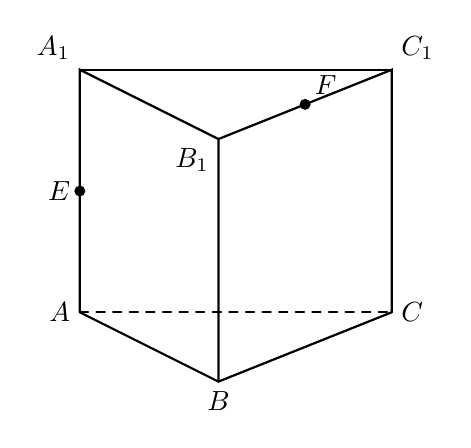
\begin{tikzpicture}[>=stealth,scale=1.1,line cap=round]
  \coordinate (A) at (0, 0.8);
  \coordinate (B) at (1.6, 0);
  \coordinate (C) at (3.6, 0.8);
  \coordinate (A1) at (0, 3.6);
  \coordinate (B1) at (1.6, 2.8);
  \coordinate (C1) at (3.6, 3.6);
  \coordinate (E) at (0, 2.2);
  \coordinate (F) at (2.6, 3.2);

  % 棱线
  \draw[thick] (A) -- (B) -- (C);
  \draw[dashed,thick] (A) -- (C);
  \draw[thick] (A) -- (A1) -- (B1) -- (B);
  \draw[thick] (B1) -- (C1) -- (C);
  \draw[thick] (A1) -- (C1);

  % 点 E, F
  \fill (E) circle (1.8pt) node[left] {$E$};
  \fill (F) circle (1.8pt) node[above right] {$F$};

  % 顶点标注
  \node[left] at (A) {$A$};
  \node[below] at (B) {$B$};
  \node[right] at (C) {$C$};
  \node[above left] at (A1) {$A_1$};
  \node[below left] at (B1) {$B_1$};
  \node[above right] at (C1) {$C_1$};
\end{tikzpicture}
